% Prof. Dr. Ausberto S. Castro Vera
% UENF - CCT - LCMAT - Curso de Ci\^{e}ncia da Computa\c{c}\~{a}o
% Campos, RJ,  2022
% Disciplina: Paradigmas de Linguagens de Programa\c{c}\~{a}o
% Aluno: Rômulo Souza Fernandes



\chapter{ Introdução}
O Python é uma linguagem orientada a objetos de alto nível que possui uma sintaxe simples e objetiva, assim colaborando para a fácil compreensão do código-fonte e permitindo que a linguagem seja produtiva. O Python contém várias estruturas de alto nível, como hora, data, dicionários, listas, complexos, entre outras estruturas, contém um amplo conjunto de módulos disponíveis para utilização, frameworks que podem ser acrescentados, possui ferramentas de outras linguagens atuais, como persistência, unidades de teste, geradores, introspecção e metaclasse, além de ter disponíveis diversas bibliotecas, como IPython, Matplotlib, mIPy, NumPy, Pandas, SciPy, ScraPy, entre outras bibliotecas conhecidas. O Python é uma linguagem multiparadigma, suportando a programação orientada a objetos, modular e funcional. A linguagem Python foi criada na Holanda, no ano de 1990, por Guido van Rossum, no Instituto Nacional de Pesquisa para Matemática e Ciência da Computação. \cite{Borges2014}


%\begin{quote}
A linguagem Python é de código aberto, porém o criador Guido van Rossum possui a função central de decidir a evolução da linguagem. O Python se popularizou e se tornou a linguagem de desenvolvimento de aplicações mais indicada para iniciantes, assim sendo aconselhada como primeira linguagem de programação.\cite{Perkovic2016}
%\end{quote}


\section{História da linguagem Python}
O intuito de Guido van Rossum era criar uma linguagem que pudesse suprir suas exigências, assim criando o Python, com base na linguagem ABC, mas solucionando as incoerências encontradas por ele na linguagem. O Python tinha como usuários principais os engenheiros e físicos.


A seguir alguns aspectos históricos da linguagem Python, baseados em\cite{Perkovic2016} e \cite{Borges2014} :
\begin{itemize}
  \item O autor principal foi o holand\^{e}s Guido van Rossum, quando trabalhava no CWI ( Centrum Wiskunde \& Informatica), em Amsterd\~{a}, Holanda.
  \item  A linguagem n\~{a}o recebeu esse nome por causada esp\'{e}cie de serpente, mas sim do seriado de com\'{e}dia da BBC \textit{Monty Python's Flying Circus} da qual Rossum \'{e} um f\~{a}.
  \item Python 0.9.0 foi lan\c{c}ado em 1991.  Esta vers\~{a}o incluia manipula\c{c}\~{a}o de exce\c{c}\~{o}es, classes, listas e strings. Tamb\'{e}m foram incl\'{\i}dos alguns aspectos de programa\c{c}\~{a}o funcional: lambda, maps flitros e reduce.
  \item  Em 1995, Guido continuou se trabalho sobre Python na Corporation for National Research Initiatives (CNRI) em Reston, Virginia, USA.
  \item Python 1.6 foi lan\c{c}ado no CNRI em
  \item  No ano 2000, Guido e a equipe de desenvolvimento principal do Python foram para BeOpen.com para formar a equipe BeOpen PythonLabs.
  \item Python 2.0 foi lan\c{c}ado no ano 2000
  \item Python 3.o foi lan\c{c}ado em dezembro de 2008
\end{itemize}

Algumas linguagens s\~{a}o consideradas  tradicionais (como mostrado na Fig.\ref{ling1}) e outras s\~{a}o consideradas modernas (ver Fig.\ref{afp}). Devemos observar aqui, que a inclus\~{a}o de qualquer figura, significa que ela deve ser referenciada em algum lugar do texto
   \begin{figure}[H]
    \begin{center}
        \caption{Logos da Linguagem Python} \label{ling1}
        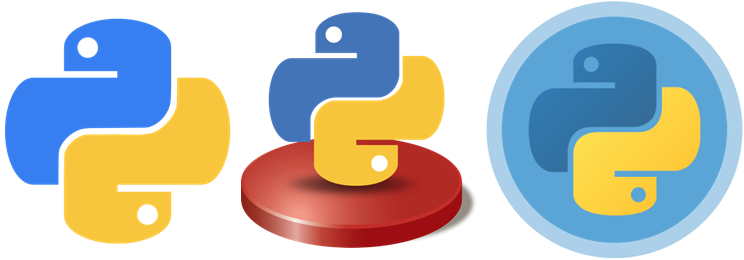
\includegraphics[width=12cm]{Python01.png} \\
        {\tiny \sf Fonte: O autor deste trabalho }
    \end{center}
   \end{figure}

Algumas figuras s\~{a}o criadas o elaboradas pelo mesmo autor, neste caso, deve-se escrever como fonte "O autor", "Os autores", etc. Figuras que incluam imagens de outras fontes deve-se especificar claramente, indicando o link o referencia correspondente, por exemplo, uma imagem que aparece em \cite[p. 93]{Sprankle2012}, \'{e} mostrada na Fig.\ref{afp} e a fonte deve ser indicada na parte inferior da figura.
   \begin{figure}[H]
    \begin{center}
        \caption{Algoritmo, Diagrama de fluxo, e Pseudo-c\'{o}digo} \label{afp}
        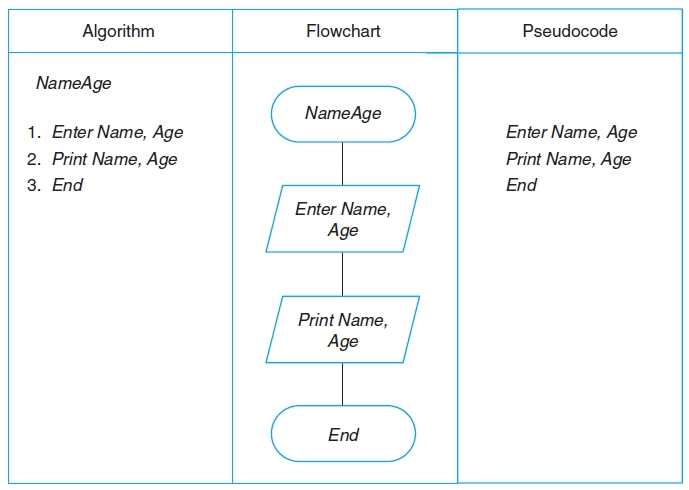
\includegraphics[width=10cm]{afp.jpg} \\
        {\tiny \sf Fonte: \cite[p. 93]{Sprankle2012} }
    \end{center}
   \end{figure}

   \section{Áreas de Aplicação da Linguagem}
   Esta linguagem \'{e} utilizada e aplicada nas seguintes \'{a}reas: !!!!! As aqui mostradas s\~{a}o exemplos!!!

        \subsection{ Big Data}
        Fazer uma breve descri\c{c}\~{a}o. Pelo menos 3 par\'{a}grafos mencionando exemplos

        \subsection{ Orientação a objetos}
        Fazer uma breve descri\c{c}\~{a}o. Pelo menos 3 par\'{a}grafos mencionando exemplos

        \subsection{ outras} 